\section{BACKGROUND: \peace\/ and d2}\label{sec:background}

\peace\/ (Parallel Environment for Assembly and Clustering of Gene
Expression) is a user-friendly nucleotide sequence clustering tool
which is designed to cluster transcript reads obtained by Sanger and
NGS sequencing technologies~\cite{rao-10,rao-18}. \peace\/ clusters
nucleotide sequences based on a Minimum Spanning Tree (MST) method as
summarized in Figure~\ref{fig:peace}.  An MST is generated (via Prim's
algorithm) using pairwise sequence comparison between the reads in
alignment-free manner using the d2 algorithm -- \ie\/ the MST edges
are weighted using d2 pseudo-metric.

\begin{figure}[h]
  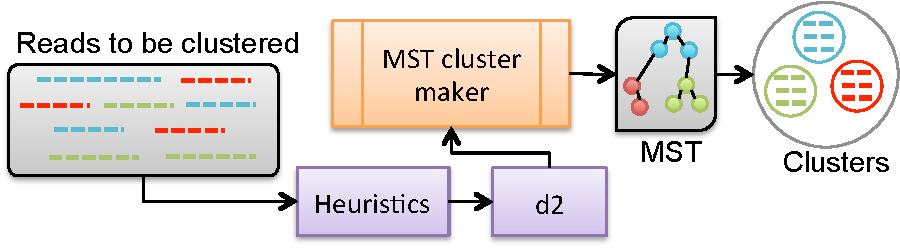
\includegraphics[width=\linewidth]{figures/peace_overview.pdf}
  \caption{Overivew of clustering in \peace}\label{fig:peace}
\end{figure}

The d2 algorithm works by comparing the frequency of words (strings of
a fixed length) appearing in a limited region of each read. \peace\/
uses a default word size of 6 base pairs. Fragments overlapping by a
sufficient length will share neighborhoods of enough similarity to
ensure a small distance (close to zero) even in the presence of a
moderate number of base errors.  Specifically, \peace\/ uses a sliding
window of fixed size $r$ (defaults to 100 in \peace) to generate d2
score for two sequences $x$ and $y$ ($|x| \ge r$, $|y| \ge r$) via:

$$
d2(x, y) = min\big\{d2(u, v) : u \sqsubseteq x, v \sqsubseteq y, |u|= |v| = r\big\}
$$

\noindent where $u \sqsubseteq x$ denotes that $u$ is a substring of
$x$. Defined as such, d2 is, in a mathematical sense, a pseudo-metric
-- \ie\/ $d2(x, y) = 0$ does not imply $x = y$.  However, as $d2(x, y)
\rightarrow 0$, $x$ is more similar to $y$ and vice versa.
Sufficiently similar reads, based on a user-defined threshold, are
clustered together.

Computing d2 distance is expensive requiring a few milliseconds for ~1
kilobase sequence.  Consequently, to minimize unsuccessful d2
comparisons, \peace\/ uses \emph{u/v} and \emph{t/v} filtering
heuristics that run in microseconds.  As indicated in
Figure~\ref{fig:peace}, the heuristics minimize the number of d2
comparisons by eliminating comparisons of sufficiently differing
sequences -- \ie\/ sequences that would result in a very high d2
distance.  A more detailed discussion on the heuristics is available
in the literature~\cite{rao-10}.

Using MST and d2, \peace\/ has shown to cluster transcript reads with
high accuracy and sensitivity. It can be run both sequentially and in
parallel, though in this study we are not exploring parallelization.
The ability to run PEACE using a Graphical User Interface and a robust
set of default/out-of-the-box parameters make it a very easy to use
tool for biologists.

\peace\/ is a highly modularized framework developed in C++ and
heavily relies on the language's object-oriented features.  The
framework consists of loosely coupled core subsystems. The subsystems
are further modularized into loosely coupled components.  Though its
modular design the framework provides the user with a wide choice of
filters, heuristics and clustering methods.  In this study, we have
used these features to implement our proposed Approximate Spanning
Tree (AST) and Prime Number-based Filter (PNF).

%% This research utilized the above mentioned PEACE framework’s
%% modularity and extensibility to develop proof of concepts for the
%% speed improvements to PEACE using Approximate Minimum Tree (AMST)
%% clustering approach and a novel Prime Number-based Filter (PNF) with a
%% few localized subsystem based additions and modifications to the PEACE
%% framework.  The clustering subsystem was modified to include the AMST
%% method (Section III.B.) and the PNF (Section III.C. ). PNF was added
%% as a component to heuristics interface and use before the use of TV
%% and UV heuristics in the heuristic chain. The improved were evaluated
%% based of runtime and clustering quality using publically available
%% nucleotide sequence data (Section III.D. ).
